%%%%\setbeamerfont{itemize/enumerate body}{size*={9}{11}}
%%%%\setbeamerfont{itemize/enumerate subbody}{size*={8}{10}}
%%%%\setbeamerfont{itemize/enumerate subsubbody}{size*={7}{9}}

\frame{%
\frametitle{Summary}
\begin{itemize}
\item Health economic evaluation
\begin{itemize}
\item What is health economics?
\item Why do we need health economics?
\end{itemize}
\item A framework for health economic evaluation
\begin{itemize}
\item Statistical modelling
\item Economic modelling
\item Decision analysis
\item Uncertainty analysis
\end{itemize}
\item Standard vs Bayesian HTA
\begin{itemize}
\item Two-stage vs integrated approach
\end{itemize}
\item Decision-making
\begin{itemize}
\item Cost-effectiveness plane
\item ICER
\item EIB
\end{itemize}
\end{itemize}

\vfill
\begin{block}{\footnotesize References}
\bmhe, chapter 1.\\
\bceabook
\end{block}

}

\frame{
\setbeamerfont{itemize/enumerate body}{size*={5}{6}}
\setbeamerfont{itemize/enumerate subbody}{size*={4}{5}}
\setbeamerfont{itemize/enumerate subsubbody}{size*={3}{4}}

\frametitle{Health technology assessment (HTA)}
\textbf{Objective}: Combine \red costs \black \& \blue benefits \black of a given intervention into a rational scheme for allocating resources
\vspace{-.4cm}
\begin{figure}
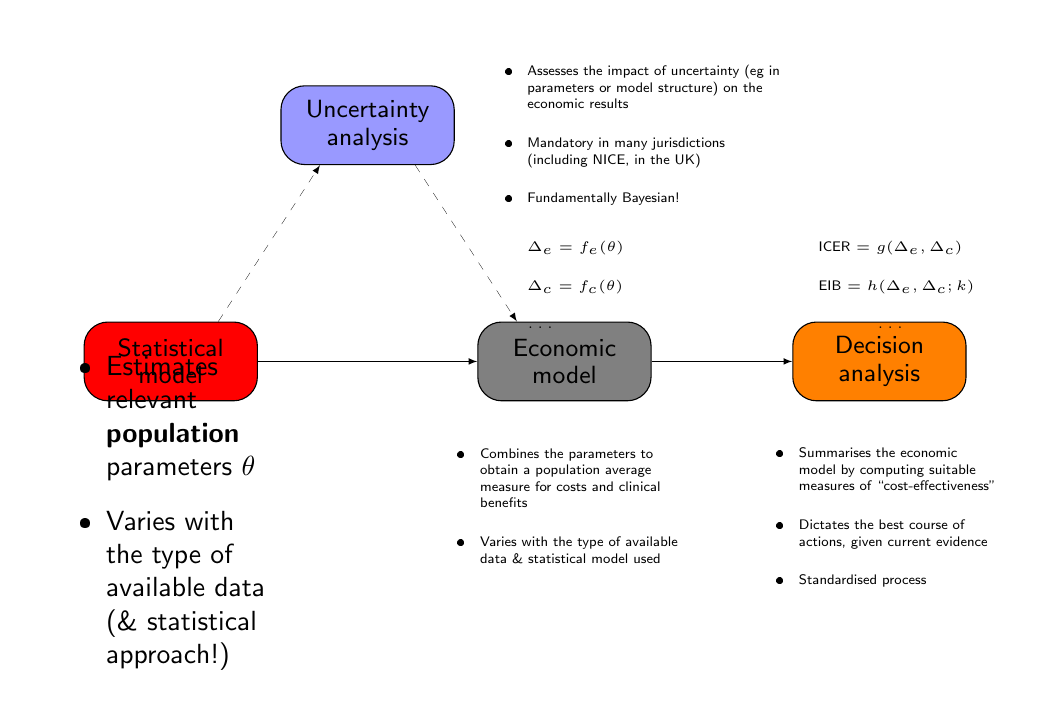
\begin{tikzpicture}%[->,>=latex,shorten >=0pt,auto,node distance=3cm,ultra thin]

\onslide<2->{\draw(-5,-1) node[align=center,rectangle,rounded corners=2ex,draw,fill=red,font=\sffamily\fontsize{9}{10}\selectfont,minimum width=2.2cm,minimum height=1cm](1){Statistical\\ model};
}
\onslide<3->{
\draw(0,-1) node[align=center,rectangle,rounded corners=2ex,draw,fill=gray,font=\sffamily\fontsize{9}{10}\selectfont,minimum width=2.2cm,minimum height=1cm](2){Economic\\ model};
}
\onslide<4->{
\draw(4,-1) node[align=center,rectangle,rounded corners=2ex,draw,fill=orange,font=\sffamily\fontsize{9}{10}\selectfont,minimum width=2.2cm,minimum height=1cm](3){Decision\\ analysis};
}
\onslide<5->{
\draw(-2.5,2) node[align=center,rectangle,rounded corners=2ex,draw,fill=blue!40,font=\sffamily\fontsize{9}{10}\selectfont,minimum width=2.2cm,minimum height=1cm](4){Uncertainty\\ analysis};
}
\onslide<2->{
\draw(-5.2,-2.7) node[align=center,rectangle,rounded corners,draw=none,font=\sffamily,text width=3cm](5){
\begin{itemize}
\item Estimates relevant \textbf{population} parameters $\bm\theta$
\item Varies with the type of available data (\& statistical approach!)
\end{itemize}
};
}
\onslide<3->{
\draw(-0.2,-2.65) node[align=center,rectangle,rounded corners,draw=none,font=\sffamily\fontsize{5}{6}\selectfont,text width=3.5cm](6){
\begin{itemize}
\item Combines the parameters to obtain a population average measure for costs and clinical benefits
\item Varies with the type of available data \& statistical model used
\end{itemize}
};
}
\onslide<4->{
\draw(3.8,-2.8) node[align=center,rectangle,rounded corners,draw=none,font=\sffamily\fontsize{5}{6}\selectfont,text width=3.4cm](7){
\begin{itemize}
\item Summarises the economic model by computing suitable measures of ``cost-effectiveness''
\item Dictates the best course of actions, given current evidence
\item Standardised process
\end{itemize}
};
}
\onslide<5->{
\draw(0.7,2.05) node[align=center,rectangle,rounded corners,draw=none,font=\sffamily\fontsize{5}{6}\selectfont,text width=4.1cm](8){
\begin{itemize}
\item Assesses the impact of uncertainty (eg in parameters or model structure) on the economic results
\item Mandatory in many jurisdictions (including NICE, in the UK)
\item Fundamentally Bayesian!
\end{itemize}
};
}
\onslide<5->{
\draw [dashed,->,>=latex,shorten >=0pt,auto,node distance=3cm,ultra thin] (1.40) -- (4.220);
\draw [dashed,->,>=latex,shorten >=0pt,auto,node distance=3cm,ultra thin] (4.320) -- (2.140);
}
\onslide<3->{
\draw [->,>=latex,shorten >=0pt,auto,node distance=3cm,ultra thin] (1.east) -- (2.west);
}
\onslide<4->{
\draw [->,>=latex,shorten >=0pt,auto,node distance=3cm,ultra thin] (2.east) -- (3.west);
}

\onslide<3->{
\draw(0.4,.15) node[align=center,rectangle,rounded corners,draw=none,font=\sffamily\fontsize{5}{6}\selectfont,text width=3.5cm](func1){
\begin{itemize}
\item[] $\myblue \Delta_e=f_e(\bm\theta)$
\item[] $\myblue \Delta_c=f_c(\bm\theta)$
\item[] $\white \ldots$
\end{itemize}
};
}

\onslide<4->{
\draw(4.1,.15) node[align=center,rectangle,rounded corners,draw=none,font=\sffamily\fontsize{5}{6}\selectfont,text width=3.5cm](func2){
\begin{itemize}
\item[] $\myblue \mbox{ICER}=g(\Delta_e,\Delta_c)$
\item[] $\myblue \mbox{EIB}=h(\Delta_e,\Delta_c;k)$
\item[] $\myblue \qquad \qquad \ldots$
\end{itemize}
};
}
\end{tikzpicture}
\end{figure}
}

\frame{
\setbeamerfont{itemize/enumerate body}{size*={5}{6}}
\setbeamerfont{itemize/enumerate subbody}{size*={4}{5}}
\setbeamerfont{itemize/enumerate subsubbody}{size*={3}{4}}

\frametitle{``Standard'' approach to HTA --- ``Two-stage''}
\begin{figure}
\begin{tikzpicture}%[->,>=latex,shorten >=0pt,auto,node distance=3cm,ultra thin]
\hspace{-.5cm}
\onslide<1->{\draw(-5,-1) node[align=center,rectangle,rounded corners=2ex,draw,fill=red,font=\sffamily\fontsize{9}{10}\selectfont,minimum width=2.2cm,minimum height=1cm](1){Statistical\\ model};
}
\onslide<1->{

\draw(0.5,-1) node[align=center,rectangle,rounded corners=2ex,draw,fill=gray,font=\sffamily\fontsize{9}{10}\selectfont,minimum width=2.2cm,minimum height=1cm](2){Economic\\ model};
}
\onslide<1->{
\draw(4,-1) node[align=center,rectangle,rounded corners=2ex,draw,fill=orange,font=\sffamily\fontsize{9}{10}\selectfont,minimum width=2.2cm,minimum height=1cm](3){Decision\\ analysis};
}
\onslide<1->{
\draw(-5,2) node[align=center,rectangle,rounded corners=2ex,draw,fill=blue!40,font=\sffamily\fontsize{9}{10}\selectfont,minimum width=2.2cm,minimum height=1cm](4){Uncertainty\\ analysis};
}
\onslide<1->{
\draw(-5.2,-2.75) node[align=center,rectangle,rounded corners,draw=none,font=\sffamily\fontsize{7}{8}\selectfont,text width=3cm](5){
\begin{itemize}
\item Estimates relevant \textbf{population} parameters $\bm\theta$
\item Varies with the type of available data (\& statistical approach!)
\end{itemize}
};
}
\onslide<1->{
\draw(0.3,-2.7) node[align=center,rectangle,rounded corners,draw=none,font=\sffamily\fontsize{7}{8}\selectfont,text width=3.5cm](6){
\begin{itemize}
\item Combines the parameters to obtain a population average measure for costs and clinical benefits
\item Varies with the type of available data \& statistical model used
\end{itemize}
};
}
\onslide<1->{
\draw(3.8,-2.85) node[align=center,rectangle,rounded corners,draw=none,font=\sffamily\fontsize{7}{8}\selectfont,text width=3.5cm](7){
\begin{itemize}
\item Summarises the economic model by computing suitable measures of ``cost-effectiveness''
\item Dictates the best course of actions, given current evidence
\item Standardised process
\end{itemize}
};
}
\onslide<1->{
\draw(-2.15,2.05) node[align=center,rectangle,rounded corners,draw=none,font=\sffamily\fontsize{7}{8}\selectfont,text width=3.7cm](8){
\begin{itemize}
\item Assesses the impact of uncertainty (eg in parameters or model structure) on the economic results
\item Mandatory in many jurisdictions (including NICE, in the UK)
\item Fundamentally Bayesian!
\end{itemize}
};
}
\onslide<1->{
%\draw [->,>=latex,shorten >=0pt,auto,node distance=3cm,ultra thin] (1.east) -- (2.west);
}
\onslide<1->{
\draw [->,>=latex,shorten >=0pt,auto,node distance=3cm,ultra thin] (2.east) -- (3.west);
}

\onslide<1->{
\draw(1.0,3.5) node[align=center,draw=none,fill=none,minimum width=.5cm,minimum height=.5cm,font=\sffamily\fontsize{6}{7}\selectfont]{\olive 1.\ Estimation (base-case)};
%\draw(4.3,3.5) node[align=center,draw=none,fill=none,minimum width=.5cm,minimum height=.5cm,font=\sffamily\fontsize{6}{7}\selectfont]{\olive 2.\ Probabilistic sensitivity analysis};
\draw(1.8,3) node[align=center,draw,fill=none,minimum width=.5cm,minimum height=.5cm,font=\sffamily\fontsize{6}{7}\selectfont](9){$\theta$};
\draw(1.8,1) node[align=center,circle,draw,fill=none,font=\sffamily\fontsize{6}{7}\selectfont](10){$y$};
\draw(.5,1) node[align=center,fill=none,minimum width=.5cm,minimum height=.5cm,font=\sffamily\fontsize{6}{7}\selectfont](11){$p(y\mid \theta)$};
\draw(.5,3) node[align=center,draw,ellipse,double,fill=none,minimum width=.3cm,minimum height=.25cm,font=\sffamily\fontsize{6}{7}\selectfont](12){$\hat\theta=f(Y)$};

\draw [->,>=latex,shorten >=0pt,auto,node distance=3cm,ultra thin] (9.south) -- (10.north);
\draw [dashed,->,>=latex,shorten >=0pt,auto,node distance=3cm,ultra thin] (11.north) -- (12.south);
\draw [dashed,->,>=latex,shorten >=0pt,auto,node distance=3cm,thin,red!60] (12.220) to [out=220,in=130] (2.120);
}

\onslide<2>{
\draw(4.3,3.5) node[align=center,draw=none,fill=none,minimum width=.5cm,minimum height=.5cm,font=\sffamily\fontsize{6}{7}\selectfont]{\olive 2.\ \textbf{Probabilistic sensitivity analysis}};
\draw(2.9,2.0) node[align=center,draw=none,fill=none,minimum width=.5cm,minimum height=.5cm,font=\sffamily\fontsize{6}{7}\selectfont,color=red]{$\Rightarrow$};
\draw(5.4,3) node[align=center,circle,draw,fill=none,font=\sffamily\fontsize{6}{7}\selectfont](13){$\theta$};
\draw(4.2,3) node[align=center,fill=none,minimum width=.5cm,minimum height=.5cm,font=\sffamily\fontsize{6}{7}\selectfont](14){$p(\theta)\red\leftrightsquigarrow\black g(\hat\theta)$};
\draw [dashed,->,>=latex,shorten >=0pt,auto,node distance=3cm,thin,blue!40] (13.south) to [out=270,in=45] (2.60);
}
\end{tikzpicture}
\end{figure}
}

\frame{
\frametitle{\only<1|handout:1>{2./3.\ Economic modelling+Decision analysis}\only<2|handout:2>{2./3./4.\ ...+\textbf{Uncertainty analysis$^*$}}}
\only<1|handout:1>{
\vspace{1.8cm}
\begin{figure}
\begin{tikzpicture}[remember picture,overlay]
\draw(0,4) node[align=center,rectangle,rounded corners,draw=none,text width=4.1cm](1){\fontsize{8}{8}\selectfont Cost-effectiveness plane};

\node{\includegraphics[scale=.55]{1.introduction-to-health-economic-evaluations/figs/CEPlane_ICER}};
\draw(3.5,-.1) node[align=center,rectangle,rounded corners,draw=none,text width=4.1cm](8){\fontsize{8}{8}\selectfont $\Delta_e$};
\draw(-.9,3.2) node[align=center,rectangle,rounded corners,draw=none,text width=4.1cm](8){\fontsize{8}{8}\selectfont $\Delta_c$};

\draw(4.5,3.5) node[align=center,rectangle,rounded corners,draw=none,text width=4.1cm](8){\fontsize{7}{8}\selectfont $\myblue \Delta_e=\red\underbrace{\myblue\mbox{E}[e \mid \hat{\bm\theta}_1]}_{\hat\mu_{e1}} \myblue - \red\underbrace{\myblue\mbox{E}[e \mid \hat{\bm\theta}_0]}_{\hat\mu_{e0}}$};
\draw(4.5,2.6) node[align=center,rectangle,rounded corners,draw=none,text width=4.1cm](8){\fontsize{7}{8}\selectfont $\myblue \Delta_c=\red\underbrace{\myblue\mbox{E}[c \mid \hat{\bm\theta}_1]}_{\hat\mu_{c1}} \myblue - \red\underbrace{\myblue\mbox{E}[c \mid \hat{\bm\theta}_0]}_{\hat\mu_{c0}}$};
\draw(2.0,1.5) node[align=center,rectangle,rounded corners,draw=none,text width=6.0cm](8){\fontsize{8}{8}\selectfont 
\begin{eqnarray*}
\mbox{ICER}&\!\!\!\!=\!\!\!\!&\frac{\mbox{E$[\Delta_c]$}}{\mbox{E$[\Delta_e]$}}=\frac{\hat\mu_{c1}-\hat\mu_{c0}}{\hat\mu_{e1}-\hat\mu_{e0}} \\
&\!\!\!\!=\!\!\!\!&\mbox{Cost per outcome}\end{eqnarray*}};
\end{tikzpicture}
\end{figure}
}

\only<2|handout:2>{
\vspace{1.8cm}
\begin{figure}
\begin{tikzpicture}[remember picture,overlay]
\draw(0,4) node[align=center,rectangle,rounded corners,draw=none,text width=4.1cm](1){\fontsize{8}{8}\selectfont Cost-effectiveness plane};
\draw(3.5,-.1) node[align=center,rectangle,rounded corners,draw=none,text width=4.1cm](8){\fontsize{8}{8}\selectfont $\Delta_e$};
\draw(-.9,3.2) node[align=center,rectangle,rounded corners,draw=none,text width=4.1cm](8){\fontsize{8}{8}\selectfont $\Delta_c$};
\node{\includegraphics[scale=.55]{1.introduction-to-health-economic-evaluations/figs/CEPlane_empty}};
\draw(4.5,3.5) node[align=center,rectangle,rounded corners,draw=none,text width=4.1cm](8){\fontsize{7}{8}\selectfont $\myblue \Delta_e=\red\underbrace{\myblue\mbox{E}[e \mid \bm{\theta}_1]}_{\mu_{e1}} \myblue - \red\underbrace{\myblue\mbox{E}[e \mid \bm{\theta}_0]}_{\mu_{e0}}$};
\draw(4.5,2.6) node[align=center,rectangle,rounded corners,draw=none,text width=4.1cm](8){\fontsize{7}{8}\selectfont $\myblue \Delta_c=\red\underbrace{\myblue\mbox{E}[c \mid \bm{\theta}_1]}_{\mu_{c1}} \myblue - \red\underbrace{\myblue\mbox{E}[c \mid \bm{\theta}_0]}_{\mu_{c0}}$};
\draw(.08,1.42) node[align=center,rectangle,rounded corners,draw=none,text width=4.1cm](8){\fontsize{5}{6}\selectfont $\red \bullet$};

\draw(-4.5,-2.6) node[align=center,rectangle,rounded corners,draw=none,text width=4.1cm](8){\fontsize{7}{8}\selectfont $^*$Induced by $\myblue g(\hat{\bm\theta}_0), g(\hat{\bm\theta}_1)$};
\end{tikzpicture}
\end{figure}
}
}

\begin{frame}[label={whatswrong}]
\frametitle{What's wrong with this?...}
\begin{itemize}
\item Potential correlation between costs \& clinical benefits \hfill\scalebox{.6}{\orange[\textbf{Individual Level + Aggregated Level Data}]}
\begin{itemize}
\item Strong positive correlation --- effective treatments are innovative and result from intensive and lengthy research $\Rightarrow$ are associated with higher unit costs
\item Negative correlation --- more effective treatments may reduce total care pathway costs e.g.\ by reducing hospitalisations, side effects, etc.
\item Because of the way in which standard models are set up, bootstrapping generally only approximates the underlying level of correlation --- \textbf{\olive MCMC does a better job!}
\end{itemize}
\vspace{10pt}\pause
\item Joint/marginal normality not realistic \hfill\scalebox{.6}{\orange[\textbf{Mainly ILD}]}
\begin{itemize}
\item Costs usually skewed and benefits may be bounded in $[0;1]$
\item Can use transformation (e.g.\ logs) --- but care is needed when back transforming to the natural scale
\item Should use more suitable models (e.g.\ Beta, Gamma or log-Normal) --- \textbf{\olive generally easier under a Bayesian framework}
\item Particularly relevant in presence of partially observed data --- more on this later!
\end{itemize}
\vspace{10pt}\pause
\item Particularly as the focus is on decision-making (rather than just inference), we need to use \textbf{all} available evidence to fully characterise current uncertainty on the model parameters and outcomes \hfill\scalebox{.6}{\orange[\textbf{Mainly ALD}]}
\begin{itemize}
\item A Bayesian approach is helpful in combining different sources of information
\item \textbf{\olive Propagating uncertainty is a fundamentally Bayesian operation!}
\end{itemize}
\end{itemize}
\end{frame}


\frame{
\setbeamerfont{itemize/enumerate body}{size*={5}{6}}
\setbeamerfont{itemize/enumerate subbody}{size*={4}{5}}
\setbeamerfont{itemize/enumerate subsubbody}{size*={3}{4}}

\frametitle{Bayesian approach to HTA --- ``Integrated''}
\begin{figure}
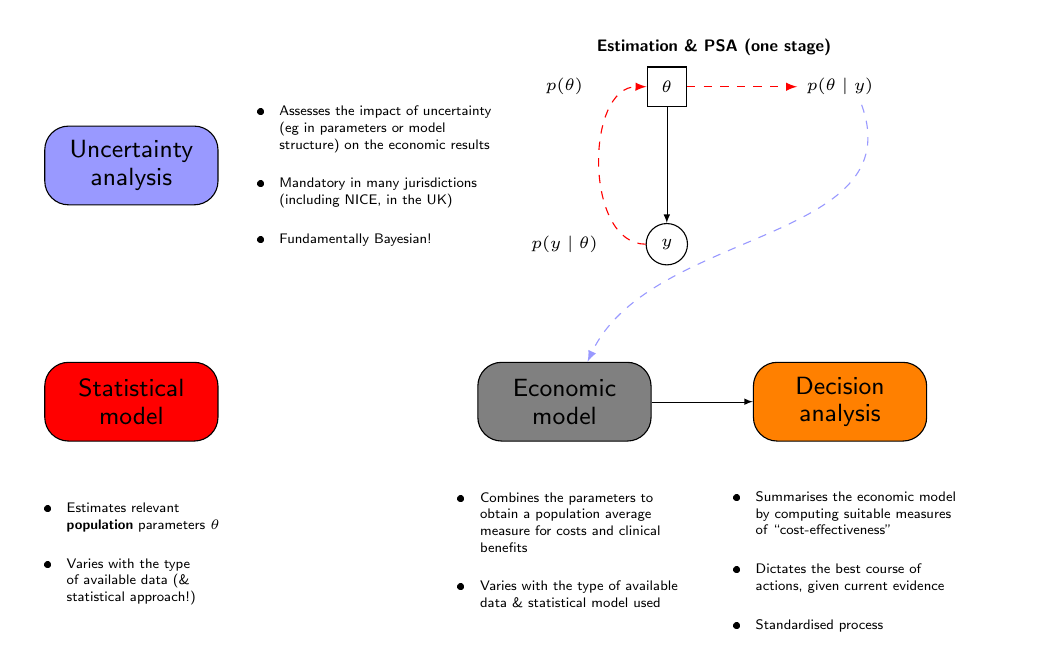
\begin{tikzpicture}%[->,>=latex,shorten >=0pt,auto,node distance=3cm,ultra thin]
\hspace{-.5cm}
\onslide<1->{\draw(-5,-1) node[align=center,rectangle,rounded corners=2ex,draw,fill=red,font=\sffamily\fontsize{9}{10}\selectfont,minimum width=2.2cm,minimum height=1cm](1){Statistical\\ model};
}
\onslide<1->{

\draw(0.5,-1) node[align=center,rectangle,rounded corners=2ex,draw,fill=gray,font=\sffamily\fontsize{9}{10}\selectfont,minimum width=2.2cm,minimum height=1cm](2){Economic\\ model};
}
\onslide<1->{
\draw(4,-1) node[align=center,rectangle,rounded corners=2ex,draw,fill=orange,font=\sffamily\fontsize{9}{10}\selectfont,minimum width=2.2cm,minimum height=1cm](3){Decision\\ analysis};
}
\onslide<1->{
\draw(-5,2) node[align=center,rectangle,rounded corners=2ex,draw,fill=blue!40,font=\sffamily\fontsize{9}{10}\selectfont,minimum width=2.2cm,minimum height=1cm](4){Uncertainty\\ analysis};
}
\onslide<1->{
\draw(-5.2,-2.75) node[align=center,rectangle,rounded corners,draw=none,font=\sffamily\tiny,text width=3cm](5){
\begin{itemize}
\item Estimates relevant \textbf{population} parameters $\bm\theta$
\item Varies with the type of available data (\& statistical approach!)
\end{itemize}
};
}
\onslide<1->{
\draw(0.3,-2.7) node[align=center,rectangle,rounded corners,draw=none,font=\sffamily\tiny,text width=3.5cm](6){
\begin{itemize}
\item Combines the parameters to obtain a population average measure for costs and clinical benefits
\item Varies with the type of available data \& statistical model used
\end{itemize}
};
}
\onslide<1->{
\draw(3.8,-2.85) node[align=center,rectangle,rounded corners,draw=none,font=\sffamily\tiny,text width=3.5cm](7){
\begin{itemize}
\item Summarises the economic model by computing suitable measures of ``cost-effectiveness''
\item Dictates the best course of actions, given current evidence
\item Standardised process
\end{itemize}
};
}
\onslide<1->{
\draw(-2.15,2.05) node[align=center,rectangle,rounded corners,draw=none,font=\sffamily\tiny,text width=3.7cm](8){
\begin{itemize}
\item Assesses the impact of uncertainty (eg in parameters or model structure) on the economic results
\item Mandatory in many jurisdictions (including NICE, in the UK)
\item Fundamentally Bayesian!
\end{itemize}
};
}
\onslide<1->{
\draw [->,>=latex,shorten >=0pt,auto,node distance=3cm,ultra thin] (2.east) -- (3.west);
}

\onslide<1->{
\draw(2.4,3.5) node[align=center,draw=none,fill=none,minimum width=.5cm,minimum height=.5cm,font=\sffamily\fontsize{6}{7}\selectfont]{\olive \textbf{Estimation \& PSA (one stage)}};
\draw(1.8,3) node[align=center,draw,fill=none,minimum width=.5cm,minimum height=.5cm,font=\sffamily\fontsize{6}{7}\selectfont](9){$\theta$};
\draw(1.8,1) node[align=center,circle,draw,fill=none,font=\sffamily\fontsize{6}{7}\selectfont](10){$y$};
\draw(.5,1) node[align=center,fill=none,minimum width=.5cm,minimum height=.5cm,font=\sffamily\fontsize{6}{7}\selectfont](11){$p(y\mid \theta)$};
\draw(.5,3) node[align=center,fill=none,minimum width=.3cm,minimum height=.25cm,font=\sffamily\fontsize{6}{7}\selectfont](12){$p(\theta)$};
\draw(4.0,3) node[align=center,fill=none,font=\sffamily\fontsize{6}{7}\selectfont](13){$p(\theta\mid y)$};

\draw [->,>=latex,shorten >=0pt,auto,node distance=3cm,ultra thin] (9.south) -- (10.north);
\draw [dashed,->,>=latex,shorten >=0pt,auto,node distance=3cm,thin,color=red] (10.180) to [bend left=90] (9.180);
\draw [dashed,->,>=latex,shorten >=0pt,auto,node distance=3cm,thin,color=red] (9.east) -- (13.west);
\draw [dashed,->,>=latex,shorten >=0pt,auto,node distance=3cm,thin,blue!40] (13.320) to [out=290,in=65] (2.60);
}
\end{tikzpicture}
\end{figure}
}


\frame{
\frametitle{\only<1|handout:1>{2./4.\ Economic modelling+Uncertainty analysis$^*$}\only<2|handout:2>{3.\ Decision analysis}}
\only<1-2>{\vspace{1.8cm}}
\begin{figure}
\begin{overprint}
\begin{tikzpicture}[remember picture,overlay]
\only<1-2|handout:1-2>{
\draw(0,4) node[align=center,rectangle,rounded corners,draw=none,text width=4.1cm](1){\fontsize{8}{8}\selectfont Cost-effectiveness plane};
}

\only<1|handout:1>{
\node{\includegraphics[scale=.55]{1.introduction-to-health-economic-evaluations/figs/CEPlane_empty}};
\draw(3.5,-.1) node[align=center,rectangle,rounded corners,draw=none,text width=4.1cm](8){\fontsize{8}{8}\selectfont $\Delta_e$};
\draw(-.9,3.2) node[align=center,rectangle,rounded corners,draw=none,text width=4.1cm](8){\fontsize{8}{8}\selectfont $\Delta_c$};
\draw(-4.0,-2.6) node[align=left,rectangle,rounded corners,draw=none,text width=4.1cm](8){\fontsize{7}{8}\selectfont $^*$Induced by $\myblue p(\bm\theta\mid \mbox{data})$};
}

\only<1-2|handout:1-2>{
\draw(4.5,3.5) node[align=center,rectangle,rounded corners,draw=none,text width=4.1cm](8){\fontsize{7}{8}\selectfont $\myblue \Delta_e=\red\underbrace{\myblue\mbox{E}[e \mid \bm{\theta}_1]}_{\mu_{e1}} \myblue - \red\underbrace{\myblue\mbox{E}[e \mid \bm{\theta}_0]}_{\mu_{e0}}$};
\draw(4.5,2.6) node[align=center,rectangle,rounded corners,draw=none,text width=4.1cm](8){\fontsize{7}{8}\selectfont $\myblue \Delta_c=\red\underbrace{\myblue\mbox{E}[c \mid \bm{\theta}_1]}_{\mu_{c1}} \myblue - \red\underbrace{\myblue\mbox{E}[c \mid \bm{\theta}_0]}_{\mu_{c0}}$};
}

\only<2|handout:2>{
\node{\includegraphics[scale=.55]{1.introduction-to-health-economic-evaluations/figs/CEPlane_ICER}};
\draw(3.5,-.1) node[align=center,rectangle,rounded corners,draw=none,text width=4.1cm](8){\fontsize{8}{8}\selectfont $\Delta_e$};
\draw(-.9,3.2) node[align=center,rectangle,rounded corners,draw=none,text width=4.1cm](8){\fontsize{8}{8}\selectfont $\Delta_c$};
\draw(2.3,1.5) node[align=center,rectangle,rounded corners,draw=none,text width=6.0cm](8){\fontsize{8}{8}\selectfont
\begin{eqnarray*}
\mbox{ICER}&\!\!\!\!=\!\!\!\!&\frac{\mbox{E$[\Delta_c]$}}{\mbox{E$[\Delta_e]$}}=\frac{\mbox{E}[\mu_{c1}]-\mbox{E}[\mu_{c0}]}{\mbox{E}[\mu_{e1}]-\mbox{E}[\mu_{e0}]} \\
&\!\!\!\!=\!\!\!\!&\mbox{Cost per outcome}
\end{eqnarray*}
};
}
\end{tikzpicture}
\end{overprint}
\end{figure}
}

\frame{
\frametitle{Decision-making based on the ICER}
\begin{overlayarea}{\textwidth}{1.5\textheight}
\begin{itemize}
\only<1|handout:1>{
\item ICER is not an ordered statistic
\begin{itemize}
\item {\color{blue}{-200/200}} better than {\color{red}{-100/200}} better than {\color{magenta}{-100/100}} in terms of decision, but ratios are -1, -1/2, -1
\item {\color{green!60!black!80} ICERs in the NW quadrant} indicate an intervention that is \textbf{dominated} (+ costs/- effectiveness)
\end{itemize}
}
\only<2|handout:2>{
\item Equivalent ICERs can mean very different things!
\begin{itemize}
\item $\color{red}(\mbox{E}[\Delta_e],\mbox{E}[\Delta_c])=(0.0005,5)$, indicates that the new treatment produces on average an increase in effectiveness of 0.0005 units at the cost of extra \pounds 10\,000
\item $\color{red!20!blue!80}(\mbox{E}[\Delta_e],\mbox{E}[\Delta_c])=(-0.0005,-5)$: new intervention less effective, but cheaper
\item In both cases, ICER = \pounds 10\,000
\end{itemize}
}
\end{itemize}
\centering
\only<1|handout:1>{
\vspace{-1.5cm}
\includegraphics[scale=.56]{1.introduction-to-health-economic-evaluations/figs/ICER_not_ordered2}
}
\only<2|handout:2>{
\includegraphics[scale=.54]{1.introduction-to-health-economic-evaluations/figs/ICER_not_int4}
}
\end{overlayarea}
}

\begin{frame}[label=decision_making]
\frametitle{Decision-theoretic approach to HTA}
\TabPositions{5.0cm}
\begin{itemize}
\item Analytic framework for decision-making in the face of uncertainty
\item Considers a set of \alert{prescriptive} axioms to ensure \textbf{rationality} in decision-making
\item Identifies the best course of action given:
\begin{itemize}
\item \alert{Model specification}
\item \alert{Current evidence}
\end{itemize}
\end{itemize}
\pause
\textbf{Process of rational decision-making}
\begin{tabular}{m{.7\textwidth}m{.3\textwidth}}
\begin{enumerate}
\item Describe uncertainty on \textit{all} unknown quantities by means of a (possibly subjective) \alert{probability distribution}
\end{enumerate}
& 
\vspace{-10pt}$\displaystyle\myblue p(\bm\omega)=p(e,c\mid\bm\theta)p(\bm\theta)$ \\[-13pt]
\begin{enumerate}\setcounter{enumi}{1}
\item For each intervention $t$, outcomes $o=(e,c)$ are valued by means of a pre-specified \alert{measure of utility}
\end{enumerate}
& 
\vspace{-10pt}$\displaystyle\myblue u(e,c;t)$ \\[-13pt]
\begin{enumerate}\setcounter{enumi}{2}
\item Select as the most ``cost-effective'' the intervention that is associated with the \alert{maximum expected utility}
\end{enumerate}
& 
\vspace{-10pt}$\displaystyle\myblue \mathcal{U}^t=\mbox{E}_{\bm\omega}[u(e,c;t)]$
\end{tabular}
\pause
\begin{itemize}
\item Typical utility function in HTA: \alert{Monetary Net Benefit} \hfill $\displaystyle\myblue u(e,c;t) = nb_t = ke_t-c_t$
\begin{itemize}
\item $k$ is the ``willingness to pay'', i.e.\ the \textit{\red cost per extra unit of effectiveness gained}
\item Fixed, \alert{linear} form, which simplifies computations
\item Assumes decision-maker is \textit{risk neutral}. Not necessarily true!
\end{itemize}
\end{itemize}
\end{frame}

\begin{frame}[label={EIB_def}]
\frametitle{ICER vs EIB}
\begin{itemize}
\item Under the MNB, the expected utility is \myblue
\begin{eqnarray*} 
\mathcal{U}^t = \mathcal{NB}_t &\!\!\!\!\!=\!\!\!\!\!& \mbox{E}{\color{blue}_{\bm\omega}}[u(e,c;t)] \\
&\!\!\!\!\!=\!\!\!\!\!& k\mbox{E}{\color{blue}_{\bm\omega}}[e_t] - \mbox{E}{\color{blue}_{\bm\omega}}[c_t] \\
&\!\!\!\!\!=\!\!\!\!\!& k\mbox{E}{\color{red}_{\bm\theta}}[e\mid \bm\theta_t]-\mbox{E}{\color{red}_{\bm\theta}}[c\mid\bm\theta_t] =  k\mbox{E}[\mu_{et}]-\mbox{E}[\mu_{ct}]
\end{eqnarray*}\black 
\textbf{NB}: The expectation is taken with respect to $p(\bm\omega)$ so $\mathcal{NB}_t$ is a pure number!

\vspace{10pt}\pause
\item Assuming we are considering only two interventions $t=(0,1)$, decision-making can be effected by looking at the \alert{Expected Incremental Benefit} \myblue
\begin{eqnarray*}
\mbox{EIB} & = & \mathcal{NB}_1-\mathcal{NB}_0 \\
& = & \left(k\mbox{E}[\mu_{e1}]-\mbox{E}[\mu_{c1}]\right) - \left(k\mbox{E}[\mu_{e0}]-\mbox{E}[\mu_{c0}]\right)\\
&=& k\mbox{E}[\Delta_e] - \mbox{E}[\Delta_c]
\end{eqnarray*}\black 

\pause\vspace{-5pt}
\item The reference treatment $t=1$ is more cost-effective than the comparator $t=0$ if \myblue
\begin{eqnarray*}
\mbox{EIB}>0 \Rightarrow k>(<)\frac{\mbox{E}[\Delta_c]}{\mbox{E}[\Delta_e]} = \mbox{ICER} \quad \mbox{if $\mbox{E}[\Delta_e]>(<)0$}
\end{eqnarray*}
\end{itemize}
\end{frame}

\frame{
\frametitle{\only<1-2|handout:1-2>{Cost-effectiveness plane vs EIB vs ICER}\only<3|handout:3>{EIB vs Willingness to pay $k$}\only<4|handout:4>{Cost effectiveness acceptability curve}}
\begin{center}
\only<1|handout:1>{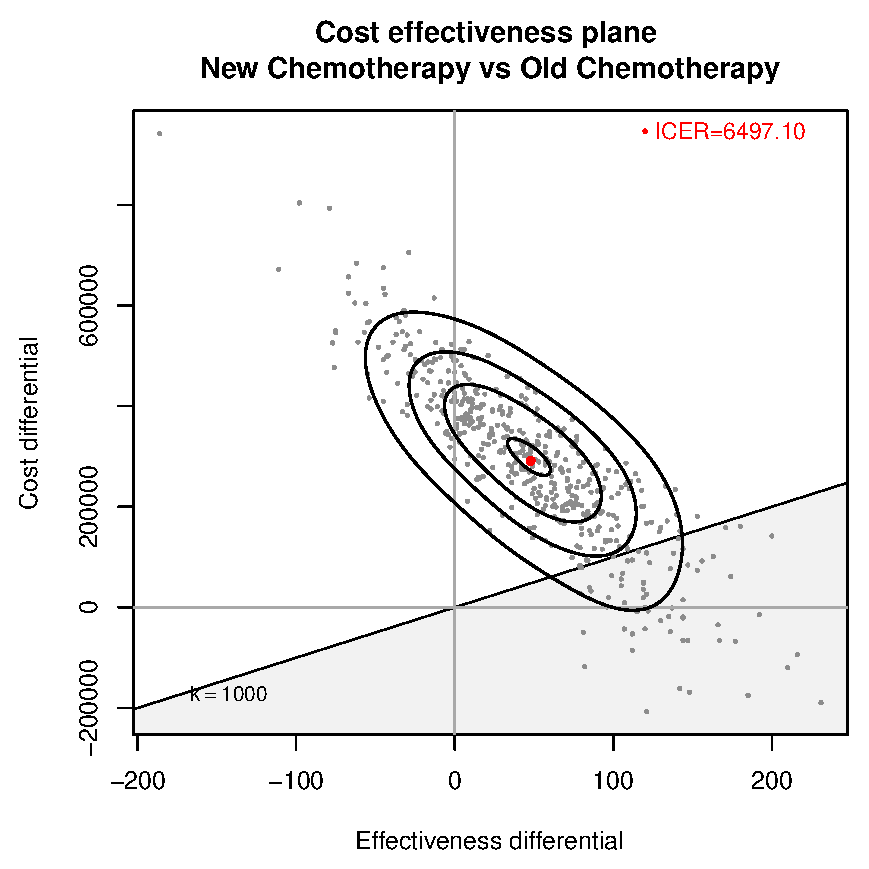
\includegraphics[width=7.6cm]{5.statistical-cost-effectiveness-analysis/figs/contour2_2}}
\only<2|handout:2>{\includegraphics[width=7.6cm]{5.statistical-cost-effectiveness-analysis/figs/contour2}}
\only<3|handout:3>{\rotatebox{0}{\includegraphics[scale=.53]{1.introduction-to-health-economic-evaluations/figs/chemo_INB}}}
\only<4|handout:4>{\includegraphics[width=7.6cm]{6.probabilistic-sensitivity-analysis/figs/CEAC}}
\end{center}
}

